\documentclass[12pt,a4paper]{article}
\usepackage[utf8]{inputenc}
\usepackage[german]{babel}
\usepackage{amsmath}
\usepackage{amsfonts}
\usepackage{amssymb}
\usepackage{graphicx}
\usepackage{enumitem}
\usepackage{gensymb}
\usepackage{wrapfig}
\usepackage{tikz}
\newcommand*\circled[1]{\tikz[baseline=(char.base)]{
            \node[color=blue,shape=circle,draw,inner sep=2pt] (char) {#1};}}
\author{Philipp Oldenburg, Patrick Zumsteg, Simon Wallny}
\title{Projekt „Sagittarius“}
\date{Herbstsemester 2014}
\begin{document}
\maketitle
\tableofcontents
\section{Vorwort}
Das Projekt „Sagittarius“, entstand im Rahmen der Vorlesung „Rechnerarchitekturen und Betriebssysteme“ an der Universität Basel im Herbstsemester 2014.\hfill\\
Die bearbeitende Gruppe besteht aus Philipp Oldenburg, Patrick Zumsteg und Simon Wallny.
\newpage
\section{Abstract (mit Resultaten)}
Im folgenden wird die Idee des Projekts beschrieben und die Anforderungen definiert. Anschließend wird auf die Umsetzung dieser Anforderungen eingegangen. Hierbei werden die Konstruktion des Roboters, die Funktionsweise der maschinellen Zielerfassung und die Interaktion zwischen den verwendeten Geräten ausgeführt. Im Anschluss werden die Resultate dargestellt:\hfill\\
Der Sagittarius ist ein fahrbarer Geschützturm mit 2 Kameras und besitzt eine Armbrust mit bis zu 4 Metern Reichweite und ausreichend hoher Präzision. Er wird über kabellose Kommunikation mit einem Laptop gesteuert. Die automatische Zielerfassung erkennt mit einem Laserpointer markierten Ziele mit $\pm$1\degree horizontaler Abweichung und berechnet die Distanz auf etwa $\pm$20cm genau.\hfill\\
Danach werden die Resultate bewertet.

\section{Projektidee}

Grundidee des Projektes war es, mit dem Lego Mindstorms-Baukasten einen Roboter zu entwerfen und zu bauen, der in der Lage ist, Ziele zu erkennen, das Objekt anzuvisieren und mit einer eingebauten Armbrust darauf zu feuern.
Ferner sollte der Roboter in der Lage sein sich zusätzlich zur Schwenkung zur Zielerfassung mithilfe einer fahrbaren Plattform zu bewegen.

Dabei war von Anfang an klar, dass wir nicht nur mit den Baukästen allein auskommen würden; vor allem deswegen, weil wir dem NXT die komplexen Operationen, die für die Zielerkennung vonnöten sind, nicht zutrauten. Folglich erweiterten wir die Projektanforderungen auch noch das Auswerten von Bildern auf dem Laptop, sowie das Entwickeln einer Software, die aufgrund dieser Daten den Roboter steuert.

\section{Umsetzung}

Das ganze Projekt lässt sich sinnvollerweise in drei thematisch grundlegend verschiedene Teile gliedern:
\begin{enumerate}
\item
Die Konstruktion des Roboters entsprechend den physischen Anforderungen.
\item
Die Zielerfassung; dazu gehört die Mustererkennung, um mit dem gewonnenen Bildmaterial ein Ziel als solches zu identifizieren, und außerdem die Berechnung der Entfernung und Position des Ziels
\item
Die Kommunikation und Interaktion zwischen Kameras, Laptop und NXT.
\end{enumerate}
Diese Dreiteilung des Projektes ermöglichte uns, einer Dreiergruppe, eine optimale Aufteilung der Arbeit. Viele Arbeitsschritte waren natürlich auf die eine oder andere Weise miteinander verbunden, und obwohl sich die Arbeitsaufträge aller Teammitglieder thematisch stark unterschieden, fanden wir uns doch sehr oft zu dritt zusammen. Dabei war es natürlich auch hilfreich, dass wir uns alle schon vor Projektbeginn kannten, was die Kommunikation und Organisation ungemein vereinfachte. 

\subsection{Konstruktion des Roboters}

\includegraphics[scale=0.1]{../Bilder/BerichtBild.png} 
Die Bestandteile des Roboters und dessen Aufbau lassen sich direkt aus den Anforderungen ableiten:
\begin{itemize}
\item
Er soll sich auf einer mobilen Plattform befinden. Hierfür eignete sich besonders eine Konstruktion, die nicht auf Rädern, sondern auf Raupen fährt, um maximale Manövrierfähigkeit zu erreichen. \circled{1}
\item
Er soll Platz für zwei Kameras \circled{2} bieten. Der Plan war ursprünglich, mit Kameras zu arbeiten, die speziell für Lego-Roboter entworfen wurden. Diese waren allerdings alle mit erheblichen Kosten belastet, und die Tatsache, dass die geplante Positionsbestimmung des Ziels sogar zwei Kameras erfordert, dazu später mehr, kam uns hier auch nicht gerade entgegen. Glücklicherweise stellte sich heraus, dass zwei Teammitglieder identische Smartphones besassen, und einer von uns hatte auch schon einige Erfahrung in der Programmierung von Android-Apps. Diese 	Smartphones werden in eigens dafür gebauten Halterungen auf beiden Seiten des Roboters quasi als „Augen“ eingesetzt.
\item
Er soll einen Geschützturm haben, der sich in horizontaler \circled{3} und in vertikaler \circled{4} Richtung orientieren lässt. Außerdem sollte der Geschützturm natürlich noch eine Konstruktion 	enthalten, mit der irgendeine Form von Projektil angemessen zielsicher verschossen werden kann. Wir haben uns hier für eine etwas modifizierte Armbrustkonstruktion entschieden; das klassische Design mit Wurfarmen, die rechtwinklig zur Schusslinie stehen, ist mit Lego schwer umzusetzen, da diese Wurfarme unter großer Spannung stehen, was die nicht besonders robusten Plastikteile vermutlich nicht ausgehalten hätten. Wir haben uns deshalb für eine inline-Konstruktion \circled{5} entschieden. Dies senkt einerseits die Spannung, unter der die Arme leiden, andererseits wird die gesamte Kraft des Gummibands dafür aufgewendet, den Bolzen zu beschleunigen. Außerdem besitzt der Wurfarm noch einen Abzug \circled{6}, der das Gummiband in gespannter Position hält und der von einem kleinen Motor ausgelöst werden 	kann.
\end{itemize}
\subsection{Zielerfassung}
Während wir zuerst geplant hatten, das Ziel durch eine bestimmte Farbe zu kennzeichnen, etwa ein roter Ballon, entschieden wir uns bei der Umsetzung doch dafür, Ziele mit einem grünen Laserpointer zu markieren. Dies erwies sich als wesentlich eleganter, da die Zielerkennung schärfer und die Anwendungsbereiche breiter wurden. 

Zur Erkennung des Laserpointers verwenden wir die OpenCV Library, mit deren Hilfe, mit etwas Aufwand, bestimmte Farbtöne erkannt, isoliert, und ihre Position bestimmt werden kann.

Der wichtigste Teil bei der Umsetzung einer Zielerfassung ist die Positionsbestimmung des markierten Objekts.
Im Einklang mit den Anforderungen einen Geschützturm auszurichten bot es sich an, die Position in Kugelkoordinaten zu erfassen, also als Vektor von Distanz, horizontaler Schwenkung und vertikaler Schwenkung.
Während die Winkel schon aus dem Bild \textit{einer} Kamera hervorgehen, ist die Bestimmung der Distanz grundlegend schwieriger. Aus den Bildern zweier Kameras dagegen lässt sich anhand der Abweichung in den Bildpositionen und den damit einhergehenden Winkeln der Abstand zum Ziel trigonometrisch bestimmen. Dabei hilft, dass die Erfassung eines Laserpointers ein sehr scharfes Ziel ist.

Nun bot es sich an die Berechnung der Position in 2 Teile aufzuteilen. Der erste Teil ermittelt die Distanz und horizontale Schwenkung anhand der X-Koordinate des Laserpunktes auf den 2 Bildern.

Dafür wird die Bildpositionen der erkannten Punkte mithilfe einer gemessenen Konstante zunächst in ein zweidimensionales,  kartesisches Hilfskoordinatensystem übertragen, in dem die Positionen der Kameras bekannt sind und der Geschützturm sich im Nullpunkt befindet. Die beiden Geraden durch die linke Kamera und den linken Bildpunkt sowie durch die rechte Kamera und den rechten Bildpunkt schneiden sich in der Position des Ziels.
\hfill\\
\hfill\\
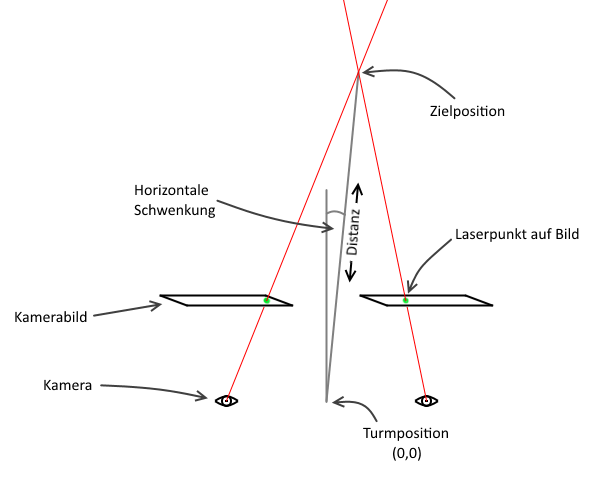
\includegraphics[scale=0.85]{../Bilder/PosBestGraph.png} 

So lässt sich die Distanz und horizontale Schwenkung aus Sicht des Turms bestimmen, und ersteres kann mithilfe einer weiteren gemessenen Konstante vom Hilfskoordinatensystem in Zentimeter transformiert werden.
Für den Schritt vom Zwei- ins Dreidimensionale fehlt noch der Vertikale Winkel. Da sich beide Kameras auf gleicher Höhe befinden liefern sie für das Ziel die gleich Höhe. (Es wird der Durchschnitt beider Werte verwendet, die sich aber nur um ein paar Pixel unterscheiden sollten). Diese kann dann vergleichsweise einfach mithilfe des gemessenen Abstands und der schon beim ersten Schritt verwendeten Konstanten in einen Winkel umgerechnet werden.

\subsection{Kommunikation}
Grundsätzlich mussten wir uns um eine Verbindung zwischen NXT und den zwei Kameras (Smartphones) kümmern. Als Vermittlungsglied soll ein Server (Laptop) dienen, welcher auch die performanceintensiven Berechnungen wie beispielsweise die Bildverarbeitung erledigt. Letztendlich haben wir uns für eine kabellose Variante entschieden:
\begin{itemize}
\item
Der NXT soll via Bluetooth mit dem Rechner verbunden werden.
\item
Die zwei Kameras sollen via WLAN mit dem Rechner kommuzieren.
\end{itemize}

\subsubsection*{NXT $\leftrightarrow$ Laptop}
\begin{wrapfigure}{R}{0.5\textwidth}
  \vspace{-40pt}
  \begin{center}
    \includegraphics[width=0.48\textwidth]{../Bilder/lejosLogo.jpg}
  \end{center}
  \vspace{-15pt}
\end{wrapfigure}
Um mit dem NXT via Bluetooth kommunizieren zu können haben wir das Framework Lejos benutzt.
Es stellt eine Firmware für den NXT bereit, welche es ermöglicht Java-Programme auszuführen.
Weiterhin gibt es Treiber für Windows-Rechner und ein Eclipse-Plugin, sodass es möglich ist über Eclipse das Programm auf den NXT zu laden und zu debuggen.
\begin{wrapfigure}{R}{0.3\textwidth}
  \vspace{-30pt}
  \begin{center}
    \includegraphics[width=0.28\textwidth]{../Bilder/Control.png}
  \end{center}
  \vspace{-15pt}
\end{wrapfigure}
Die Installation ist sehr mühsam, da die Treiber für den NXT viele Abhängigkeiten haben und nicht weiterentwickelt werden. Die neueste, von Lego bereitgestellte Distribution eines solchen Treibers ist sogar bekannterweise fehlerhaft, und wir mussten als Workaround eine third-party-Software verwenden, die allerdings den gleichen Zweck erfüllt.
Lejos-Schnittstellen laufen nur unter 32-bit Anwendungen (Eclipse, Java).

Trotz alledem stellt Lejos sehr einfache Schnittstellen zur Verfügung, mit denen es einem möglich ist, ohne Probleme Motoren zu steuern und eine Bluetooth-Verbindung aufzubauen.
Ein kleines Interface ermöglicht es dem Benutzer den Roboter zu steuern:
\begin{enumerate}
\item Via UP, LEFT, DOWN, RIGHT lässt sich der Roboter steuern
\item „BTCONNECT“, „Disc“ dienen dazu den Server mit dem Roboter zu verbinden/ zu trennen.
\item „Send Pic“ fordert Bilder der Kameras an
\end{enumerate}
\newpage


\subsubsection*{Laptop $\leftrightarrow$ Kameras}
\begin{wrapfigure}{R}{0.2\textwidth}
  \vspace{-40pt}
  \begin{center}
    \includegraphics[width=0.18\textwidth]{../Bilder/Android-Logo.png}
  \end{center}
  \vspace{-20pt}
\end{wrapfigure}
Als Kameras dienen uns zwei Samsung Galaxy S2 (Android Version 4.1.2).
Um eine stabile Kommunikation zu gewährleisten haben wir uns für eine Server-Client-Architektur entschieden, welche wir schon aus dem Programmierprojekt kennen.
Ein kleines Protokoll hilft uns eine Synchronisation der Kameras zu gewährleisten.
Etwas vereinfacht sieht die Vorgehensweise folgendermassen aus:
\begin{enumerate}
\item
Server befehligt Kameras zu Fokusierung
\item
Kameras melden zurück bei Erfolg
\item
Sobald der Server ein „OK“ von beiden Kameras erhalten hat, wird der Befehl zum Foto schießen gesendet
\end{enumerate}

Auf dem Rechner werden die erhaltenen Fotos in einer GUI dargestellt und nach einer Mustererkennung ausgewertet.

\subsubsection*{Lessons Learned Kommunikation}
Die drahtlose Übertragung ist zum einen must-have für einen mobilen Roboter, doch andererseits führt dies zu Einbußen in der Übertragungsgeschwindigkeit. Die Übertragung der zwei Kamerabilder nimmt einige Sekunden in Anspruch. Dies ist aber prinzipiell kein Problem, da unser Roboter keine schnellen Reflexe im Kampf benötigt.

Es ist erstaunlich, wie viel Aufwand erforderlich ist, um mehrere Hardwarekomponenten miteinander zu verbinden und eine stabile Kommunikation zwischen diesen zu etablieren. Es lässt sich mit Sicherheit sagen, dass das Projekt noch um ein Vielfaches aufwendiger geworden wäre, wenn uns die früher genannten Frameworks und Schnittstellen-Softwares nicht zur Verfügung gestanden hätten.

\section{Resultate}
Der Roboter selbst erfüllt alle Anforderungen, die ursprünglich gestellt wurden. Die effektive Reichweite beträgt bei maximalem Abschusswinkel etwa 4 Meter. 
Sowohl die Bewegung auf den Raupen als auch die horizontale Ausrichtung des Geschützturms ist sehr präzise, und kann die Genauigkeit der Bildauswertung 
vollkommen nutzen. Die vertikale Ausrichtung ist etwas weniger präzise, und auf ungefähr 20\degree limitiert. Allerdings ist dies auch kein grosses Problem, da 
das Projektil auch bei grösseren Entfernungen nicht sonderlich stark abfällt. Das Verschiessen von Holzspiessen, die einen Ballon effektiv zum Platzen gebracht
hätten, war uns leider nicht möglich. Stattdessen verschiessen wir Lego-Verstrebungen, die zwar keine Spitze haben, aber trotzdem eine durchaus adäquate Menge
an Energie an ihr Ziel abgeben.\hfill\\
\hfill\\
Der Zielerfassungsalgorithmus war in der Lage in mehreren Tests den Winkel auf eine Abweichung von unter $\pm$ 1\degree zu bestimmen.
Die genaue Distanz zu bestimmen erwies sich als deutlich schwieriger, allerdings, nach Kalibrierung anhand zahlreicher Tests, konnten wir die Abweichung bei 1-3m auf etwa $\pm$ 20cm beschränken.

\section{Bewertung und Ausblick}
Wir sind mit unseren Resultaten insgesamt zufrieden.\hfill\\
Die Zielerkennung erwies sich wie erwartet als schwierig, jedoch haben wir nach nennenswertem Aufwand einen Algorithmus geschrieben der falsche Positive und falsche negative minimal hält. Ohne die OpenCV Library wäre uns das allerdings nicht möglich gewesen.\hfill\\
Bei der Konstruktion des Roboters mussten wir einige Abstriche machen, weil das Material den physischen Ansprüchen nicht gerecht wurde, aber nachdem wir uns auf ein realistisches Maß geeinigt hatten haben wir eine zufriedenstellende Maschine erstellt.\hfill\\
Die Integration von Smartphones und Laptops in das Projekt war zunächst tückisch aber konnte gut bewältigt werden.

\end{document}